\section{Superblock distributions in deployed cryptocurrencies}

We measured the superblock distribution in the mainnet Bitcoin blockchain. Our
results are illustrated in Figure~\ref{fig.btc-bch-superblocks}. As expected,
half the blockchain blocks are $1$-superblocks, $1/4$ of blocks are
$2$-superblocks and generally approximately $2^{-\mu}$ of the blockchain blocks
are $\mu$-superblocks. The figure also shows the superblock distribution for
Bitcoin Cash, which deviates from Bitcoin's after the fork. The figure shows
that the size of the interlink vector is increasing at a logarithmic rate. The
horizontal axis denotes the block height in log-scale, while the vertical axis
denotes the size of the interlink vector $|\textsf{interlink}|$ when corrected
for variable difficulty by the mining power correction term
$+ \log_2(\frac{\textsf{variableTarget}}{\textsf{genesisTarget}})$, where
$\textsf{variableTarget}$ denotes the difficulty-adjusted mining target
and $\textsf{genesisTarget}$ denotes the target of the genesis block (and note
that this term will be negative). The block height up to the first $10^3$ blocks
are dominated by Genesis, which happened to be a $12$-superblock. The plot can
be decreasing due to increasing difficulty, which makes the correction parameter
more negative. The plot for Bitcoin Cash is increasing due to decreased
difficulty after the fork.

\begin{figure*}[h]
\begin{center}
  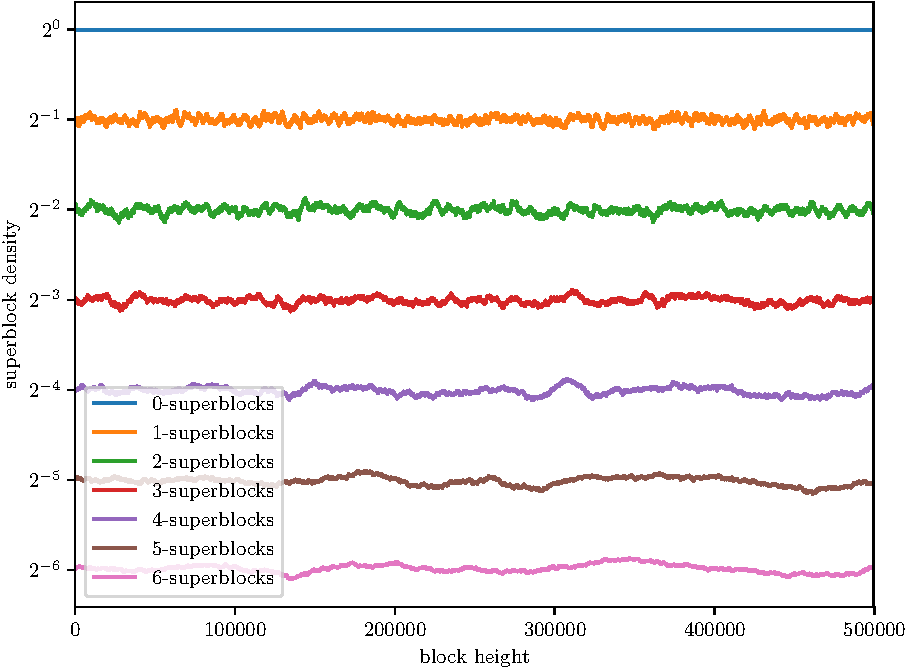
\includegraphics[width=0.95\textwidth]{figures/bitcoin-superblock-distribution.pdf}
  \caption{The distribution of block levels in Bitcoin and Bitcoin Cash. The
           graph has been corrected to account for variable difficulty. Block
           height in log-scale.}
  \label{fig.btc-bch-superblocks}
  \end{center}
\end{figure*}
